\documentclass{beamer}
\usetheme{Warsaw}
\setbeamertemplate{headline}{}

\usepackage{ae,lmodern}
\usepackage[english]{babel}
\usepackage[utf8]{inputenc}
\usepackage[T1]{fontenc}

\usepackage{caption}
\captionsetup[figure]{labelformat=empty}

\PassOptionsToPackage{usenames,dvipsnames}{xcolor}
\usepackage{xcolor,colortbl}
\definecolor{DarkGrey}{HTML}{222222}
\definecolor{DarkBlue}{HTML}{004BA9}
\definecolor{DarkRed}{HTML}{CC1111}
\definecolor{DarkGreen}{HTML}{117711}
\definecolor{DarkOrange}{HTML}{CC7000}
\definecolor{LightGrey}{HTML}{DDDDDD}
\definecolor{LightBlue}{HTML}{F0F8FF}
\definecolor{codegreen}{rgb}{0,0.6,0}
\definecolor{codepurple}{rgb}{0.58,0,0.82}

\usepackage[cache=false]{minted}
\setminted[bash]{
   bgcolor=LightBlue,
   breaklines, breakanywhere,
   frame=single,
   autogobble
}
\usemintedstyle[python]{native}
\setminted[python]{
   bgcolor=black,
   breaklines, breakanywhere,
   autogobble
}

\usepackage{listings}
\usepackage{lstautogobble}
\lstdefinestyle{bash}{
    backgroundcolor=\color{DarkGrey},   
    commentstyle=\color{codegreen},
    keywordstyle=\color{magenta},
    numberstyle=\tiny\color{DarkGrey},
    stringstyle=\color{codepurple},
    basicstyle=\ttfamily\tiny\color{LightGrey},
    escapeinside={\%*}{*)},
    breakatwhitespace=false,         
    breaklines=true,                 
    captionpos=b,                    
    keepspaces=true,                 
    numbers=left,                    
    numbersep=5pt,                  
    showspaces=false,                
    showstringspaces=false,
    showtabs=false,
    showlines=false,
    tabsize=2
}

\usepackage{tikz}
\usetikzlibrary{calc,decorations.pathreplacing,arrows,arrows.meta,shapes,patterns, positioning}
\newcommand\BigLength{14.6em}
\newcommand\Height{2em}
\newcommand\Sep{0.6em}
\newcommand\Center{\BigLength*1/2}
\newcommand\BigBox{\BigLength+\Sep}
\newcommand\HalfBox{\BigLength*1/2-\Sep*1/4}
\newcommand\HalfLength{\BigLength*1/2-\Sep*5/4}
\newcommand\CenterL{\BigLength*1/4-\Sep*1/8}
\newcommand\CenterR{\BigLength*3/4+\Sep*1/8}
\tikzstyle{layer}=[rectangle,thick,text centered,
                     minimum height=\Height,minimum width=\BigLength]
\tikzstyle{short}=[rectangle,thick,text centered,
                     minimum height=\Height,minimum width=\HalfLength]
\tikzstyle{dibox}=[rectangle,thick,semitransparent,
                     minimum height=(\Height+\Sep)*2,minimum width=\BigBox]
\tikzstyle{vmbox}=[rectangle,thick,semitransparent,
                     minimum height=(\Height+\Sep)*3,minimum width=\HalfBox]
\tikzstyle{ctbox}=[rectangle,thick,semitransparent,
                     minimum height=(\Height+\Sep)*2,minimum width=\HalfBox]
\tikzstyle{vebox}=[rectangle,thick,semitransparent,
                     minimum height=(\Height+\Sep)*1,minimum width=\HalfBox]

\usepackage{hyperref}
\usepackage{grffile}


\AtBeginSection[]
{
   \begin{frame}
      \tableofcontents[currentsection]
   \end{frame}
}

\AtBeginSubsection[]
{
   \begin{frame}
      \tableofcontents[currentsection, currentsubsection, sectionstyle=shaded]
   \end{frame}
}

%----------------------------------------------------------------------------------------
\title{Introduction to Data Science}
\subtitle{with Python}
%----------------------------------------------------------------------------------------
\author{Alexis Bogroff}
\date{\today}



\newlength\myheight
\newlength\mydepth
\settototalheight\myheight{Xygp}
\settodepth\mydepth{Xygp}
\setlength\fboxsep{0pt}
\newcommand*\inlinegraphics[1]{%
  \settototalheight\myheight{Xygp}%
  \settodepth\mydepth{Xygp}%
  \raisebox{-\mydepth}{\includegraphics[height=\myheight]{#1}}%
}

\begin{document}

\begin{frame}
   \titlepage
\end{frame}

\begin{frame}\frametitle{Presenter}
   \begin{minipage}{0.3\linewidth}
      \centering
      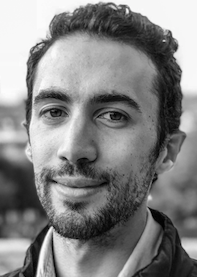
\includegraphics[width=0.6\textwidth]{../images/AlexisBogroff.png} \\
   \end{minipage}
   \begin{minipage}{0.6\linewidth}
      \noindent Alexis Bogroff \\
      Lecturer and Mentor in Data Science \\
      at Paris 1 Panthéon-Sorbonne, ESILV, Openclassrooms, EM-Lyon
   \end{minipage}
   \\[2ex]
   \visible<2->{\begin{itemize}
      \item 4 years Teaching Assistant and lecturer in VBA, Python for finance, SQL, Data Analysis and Data Science
      \item 9 months Researcher Assistant at Paris 1 Panthéon-Sorbonne within H2020 European Project
      \item 1 year Data Scientist at Pléiade Asset Management
   \end{itemize}}
   \hfill
\end{frame}

% \begin{frame}\frametitle{Overview}
%    \Large
%    \centering
%    Financial Engineering with Python Linux and Git \\[2ex]
%    \begin{minipage}{0.32\linewidth}
%       \includegraphics[width=0.8\textwidth]{../images/linux-1-logo-svg-vector.pdf}
%    \end{minipage}
%    \begin{minipage}{0.32\linewidth}
%       \includegraphics[width=0.8\textwidth]{../images/Git-logo.pdf}
%    \end{minipage}
%    \begin{minipage}{0.32\linewidth}
%       \includegraphics[width=0.9\textwidth]{../images/Python_logo_and_wordmark.pdf}
%    \end{minipage}
%    \pause
%    \\[3ex]
%    Free and everywhere stack \\
%    To find a job and be operational
% \end{frame}

% \begin{frame}\frametitle{Lecture Organisation}
%    \begin{itemize}[<+->]
%       \item Prerequisite:
%       \begin{enumerate}
%          \item Have a Linux environment working on your personal computer
%          \item[] (it can be WSL2 on Windows, Amazon EC2 for a distant solution)
%          \item Install Git
%          \item Install Python
%       \end{enumerate}
%       \vspace{2em}
%       \item Exam:
%       \begin{itemize}
%          \item Last QCM 1/2
%          \item Project 1/2
%       \end{itemize}
%    \end{itemize}
% \end{frame}


\begin{frame}
   \tableofcontents
\end{frame}

% =============================================================================
% =============================================================================
\section{Python Programming}
% 3 Hours course
% =============================================================================
% =============================================================================


%------------------------------------------------------------------------------
\subsection{Why Python?}
%------------------------------------------------------------------------------

\begin{frame}\frametitle{Why Python?}
   \begin{itemize}
      \item Versatile
      \item Simple
      \item Open Source
      \item Most used for Data Science
   \end{itemize}

   \vspace{1cm}
   \begin{minipage}{0.4\linewidth}
      \begin{figure}[H]
         
\includegraphics[width=2.5cm]{../images/illustrations/python_logo.png}
      \end{figure}
   \end{minipage}

\end{frame}


%------------------------------------------------------------------------------
\subsection{Programming Environment}
%------------------------------------------------------------------------------
\begin{frame}\frametitle{Programming Environment}

   \begin{minipage}{0.4\linewidth}
      \begin{itemize}
         \item Interactive console   
      \end{itemize}
   \end{minipage}
   \begin{minipage}{0.58\linewidth}
      \begin{figure}[H]
         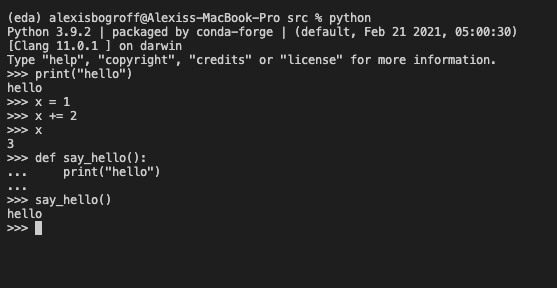
\includegraphics[width=6cm]{../images/illustrations/interactive_console.jpg}
      \end{figure}
   \end{minipage}
\end{frame}



\begin{frame}\frametitle{Programming Environment}

   \begin{minipage}{0.4\linewidth}
      \begin{itemize}
         \item Interactive console   
         \item Scripts
      \end{itemize}
   \end{minipage}
   \begin{minipage}{0.58\linewidth}
      \begin{figure}[H]
         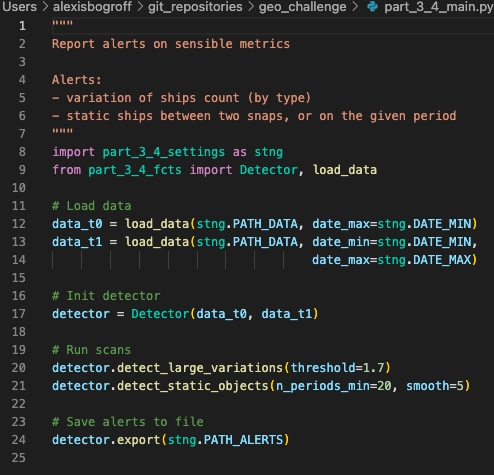
\includegraphics[width=5.5cm]{../images/illustrations/script.jpg}
      \end{figure}
      \begin{figure}[H]
         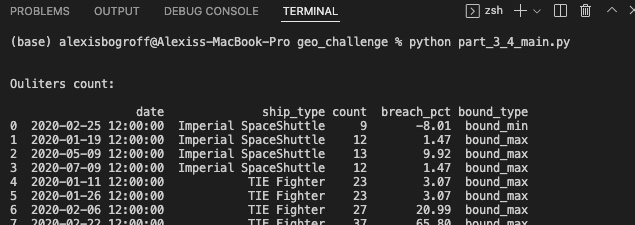
\includegraphics[width=5.5cm]{../images/illustrations/launch_script.jpg}
      \end{figure}
   \end{minipage}
\end{frame}


\begin{frame}\frametitle{Programming Environment}

   \begin{minipage}{0.4\linewidth}
      \begin{itemize}
         \item Interactive console   
         \item Scripts
         \item Jupyter Notebooks
      \end{itemize}
   \end{minipage}
   \begin{minipage}{0.58\linewidth}
      \begin{figure}[H]
         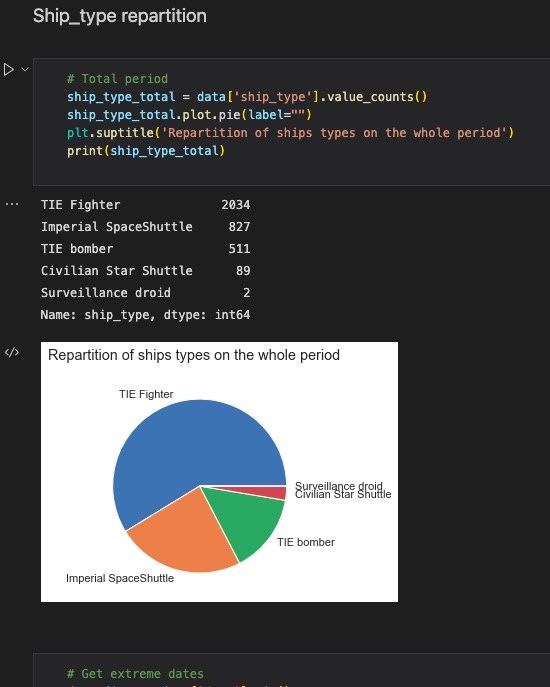
\includegraphics[width=6cm]{../images/illustrations/notebook.jpg}
      \end{figure}
   \end{minipage}
\end{frame}


\begin{frame}\frametitle{Programming Environment}

   \begin{minipage}{0.4\linewidth}
      \begin{itemize}
         \item Interactive console   
         \item Scripts
         \item Jupyter Notebooks
         \item Code editors\\(VS Code)
      \end{itemize}
   \end{minipage}
   \begin{minipage}{0.58\linewidth}
      \begin{figure}[H]
         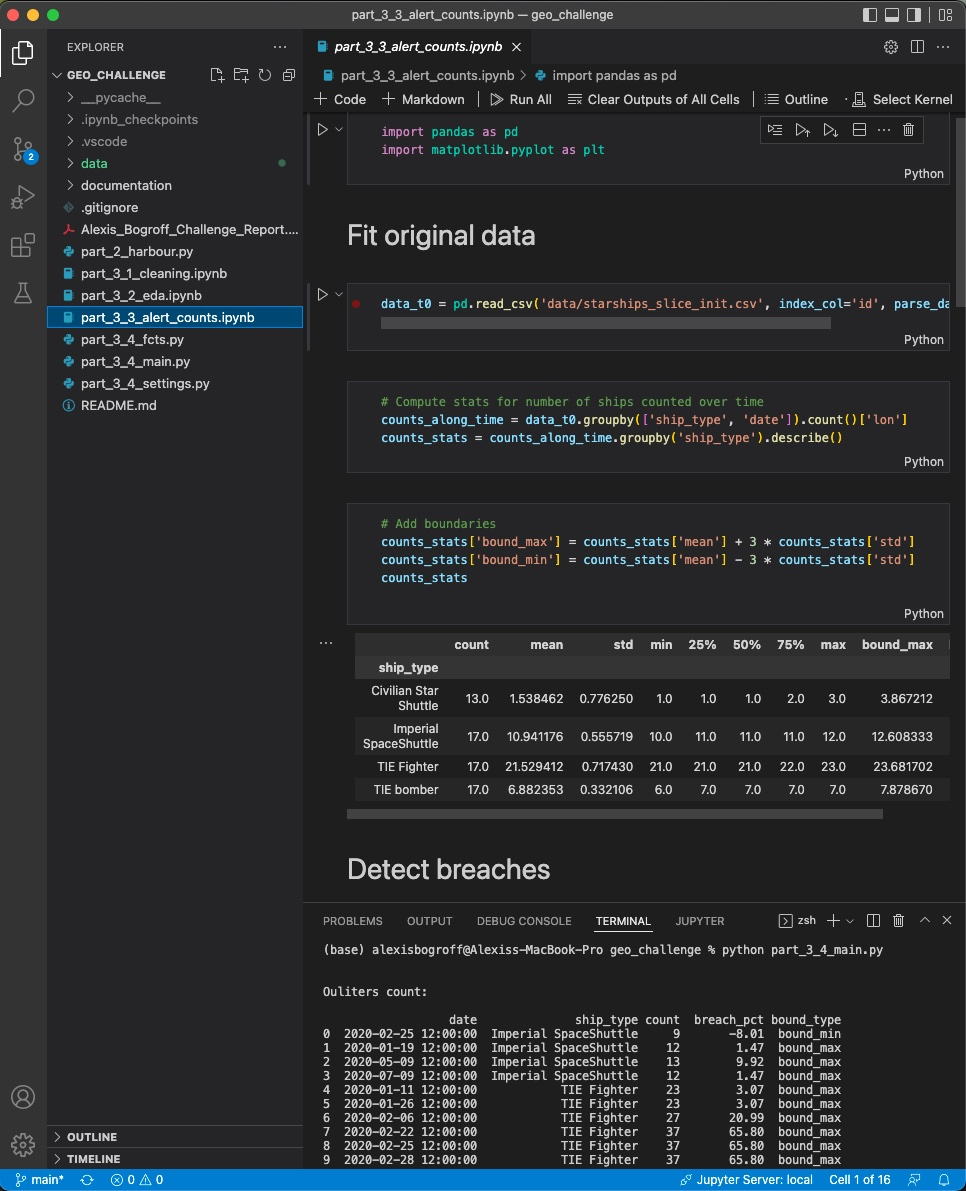
\includegraphics[width=6cm]{../images/illustrations/vscode.jpg}
      \end{figure}
   \end{minipage}
\end{frame}



\begin{frame}\frametitle{Programming Environment}

   \begin{minipage}{0.4\linewidth}
      \begin{itemize}
         \item Interactive console   
         \item Scripts
         \item Jupyter Notebooks
         \item Code editors\\(VS Code)
         \item Packages managers\\(Conda, Pip)
      \end{itemize}
   \end{minipage}
   \begin{minipage}{0.58\linewidth}
      \begin{figure}[H]
         
\includegraphics[width=6cm]{../images/illustrations/pip.png}
      \end{figure}
      \begin{figure}[H]
         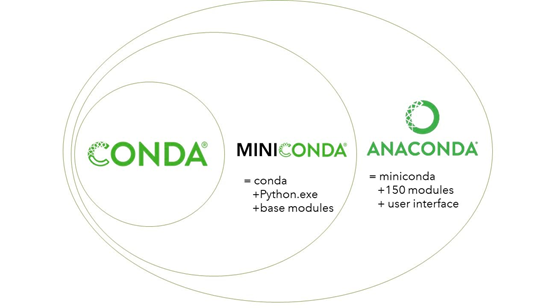
\includegraphics[width=6cm]{../images/illustrations/conda.png}
      \end{figure}
   \end{minipage}
\end{frame}



\begin{frame}\frametitle{Programming Environment}

   \begin{minipage}{0.4\linewidth}
      \begin{itemize}
         \item Interactive console   
         \item Scripts
         \item Jupyter Notebooks
         \item Code editors\\(VS Code)
         \item Packages managers\\(Conda, Pip)
         \item Packages / Libraries\\(Pandas, Matplotlib)
      \end{itemize}
   \end{minipage}
   \begin{minipage}{0.58\linewidth}
      \begin{figure}[H]
         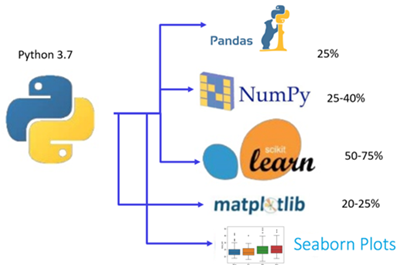
\includegraphics[width=6cm]{../images/illustrations/packages.png}
      \end{figure}
   \end{minipage}
\end{frame}


\begin{frame}\frametitle{Programming Environment}

   \begin{minipage}{0.48\linewidth}
      \begin{itemize}
         \item Interactive console   
         \item Scripts
         \item Jupyter Notebooks
         \item Code editors\\(VS Code)
         \item Packages managers\\(Conda, Pip)
         \item Packages / Libraries\\(Pandas, Matplotlib)
         \item Virtual Environments
      \end{itemize}
   \end{minipage}
   \begin{minipage}{0.5\linewidth}
      \begin{itemize}
         \item Virtualenv
         \item Pipenv
         \item Venv
         \item Poetry
      \end{itemize}
   \end{minipage}
\end{frame}


\begin{frame}\frametitle{Programming Environment}

   \begin{minipage}{0.48\linewidth}
      \begin{itemize}
         \item Interactive console   
         \item Scripts
         \item Jupyter Notebooks
         \item Code editors\\(VS Code)
         \item Packages managers\\(Conda, Pip)
         \item Packages / Libraries\\(Pandas, Matplotlib)
         \item Virtual Environments
         \item Version Control Systems\\(Git, Github, Gitlab)
      \end{itemize}
   \end{minipage}
   \begin{minipage}{0.5\linewidth}
      \begin{figure}[H]
         
\includegraphics[width=4cm]{../images/illustrations/git.png}
      \end{figure}
      \begin{figure}[H]
         
\includegraphics[width=4cm]{../images/illustrations/github.png}
      \end{figure}
      \begin{figure}[H]
         
\includegraphics[width=4cm]{../images/illustrations/gitlab.png}
      \end{figure}
   \end{minipage}
\end{frame}


%------------------------------------------------------------------------------
\subsection{Essentials in the Python language}
%------------------------------------------------------------------------------

\begin{frame}\frametitle{Essentials in the Python language}

   \begin{itemize}
      \item Data types and structures
      \begin{itemize}
         \item Numbers
         \item Text (strings)
         \item Iterables
         \item Other
      \end{itemize}
   \end{itemize}

   \begin{figure}[H]
      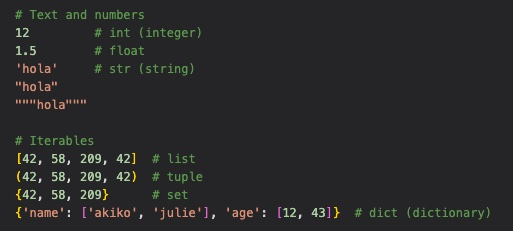
\includegraphics[width=8cm]{../images/illustrations/python_types.jpg}
   \end{figure}
\end{frame}


\begin{frame}\frametitle{Essentials in the Python language}
   \begin{minipage}{0.48\linewidth}
      \begin{itemize}
         \item Operators
         \begin{itemize}
            \item Greater than, lower than
         \end{itemize}
      \end{itemize}
   \end{minipage}
   \begin{minipage}{0.48\linewidth}
      \begin{figure}[H]
         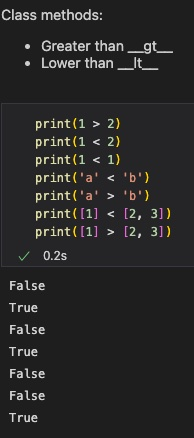
\includegraphics[width=3cm]{../images/illustrations/gt_lt.jpg}
      \end{figure}
   \end{minipage}
\end{frame}

\begin{frame}\frametitle{Essentials in the Python language}
   \begin{minipage}{0.48\linewidth}
      \begin{itemize}
         \item Operators
         \begin{itemize}
            \item Greater than, lower than
            \item Greater or equal than, lower or equal than
         \end{itemize}
      \end{itemize}
   \end{minipage}
   \begin{minipage}{0.48\linewidth}
      \begin{figure}[H]
         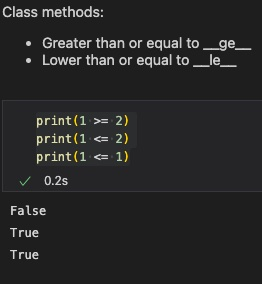
\includegraphics[width=4cm]{../images/illustrations/ge_le.jpg}
      \end{figure}
   \end{minipage}
\end{frame}

\begin{frame}\frametitle{Essentials in the Python language}
   \begin{minipage}{0.48\linewidth}
      \begin{itemize}
         \item Operators
         \begin{itemize}
            \item Greater than, lower than
            \item Greater or equal than, lower or equal than
            \item Equals to, different from
         \end{itemize}
      \end{itemize}
   \end{minipage}
   \begin{minipage}{0.48\linewidth}
      \begin{figure}[H]
         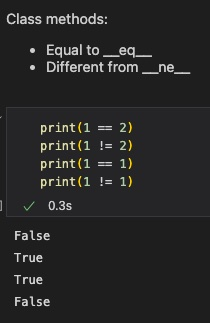
\includegraphics[width=3.2cm]{../images/illustrations/eq_ne.jpg}
      \end{figure}
   \end{minipage}
\end{frame}

\begin{frame}\frametitle{Essentials in the Python language}
   \begin{minipage}{0.48\linewidth}
      \begin{itemize}
         \item Operators
         \begin{itemize}
            \item Greater than, lower than
            \item Greater or equal than, lower or equal than
            \item Equals to, different from
            \item in
         \end{itemize}
      \end{itemize}
   \end{minipage}
   \begin{minipage}{0.48\linewidth}
      \begin{figure}[H]
         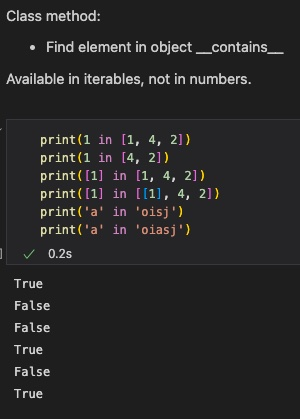
\includegraphics[width=4.5cm]{../images/illustrations/in.jpg}
      \end{figure}
   \end{minipage}
\end{frame}

\begin{frame}\frametitle{Essentials in the Python language}
   \begin{minipage}{0.48\linewidth}
      \begin{itemize}
         \item Operators
         \begin{itemize}
            \item Greater than, lower than
            \item Greater or equal than, lower or equal than
            \item Equals to, different from
            \item in
            \item not
         \end{itemize}
      \end{itemize}
   \end{minipage}
   \begin{minipage}{0.48\linewidth}
      \begin{figure}[H]
         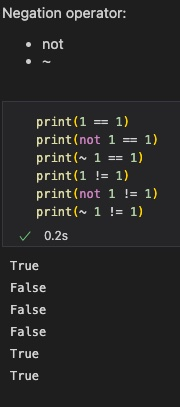
\includegraphics[width=2.6cm]{../images/illustrations/not.jpg}
      \end{figure}
   \end{minipage}
\end{frame}

\begin{frame}\frametitle{Essentials in the Python language}
   \begin{minipage}{0.48\linewidth}
      \begin{itemize}
         \item Operators
         \begin{itemize}
            \item Greater than, lower than
            \item Greater or equal than, lower or equal than
            \item Equals to, different from
            \item in
            \item not
            \item is
         \end{itemize}
      \end{itemize}
   \end{minipage}
   \begin{minipage}{0.48\linewidth}
      \begin{figure}[H]
         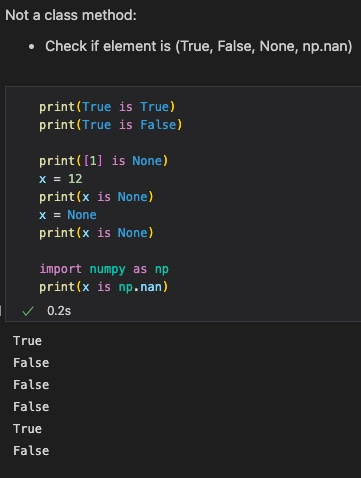
\includegraphics[width=4.5cm]{../images/illustrations/is.jpg}
      \end{figure}
   \end{minipage}
\end{frame}


\begin{frame}\frametitle{Essentials in the Python language}
   \begin{minipage}{0.48\linewidth}
      \begin{itemize}
         \item Conditional structures
         \begin{itemize}
            \item if else statement
         \end{itemize}
      \end{itemize}
   \end{minipage}
   \begin{minipage}{0.48\linewidth}
      \begin{figure}[H]
         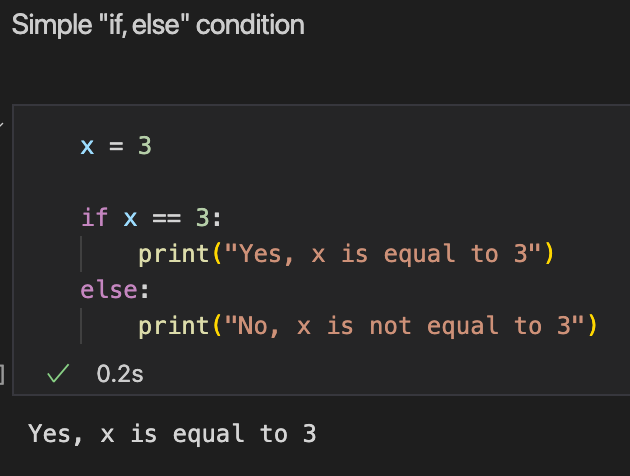
\includegraphics[width=4.5cm]{../images/illustrations/if_else.png}
      \end{figure}
   \end{minipage}
\end{frame}


\begin{frame}\frametitle{Essentials in the Python language}
   \begin{minipage}{0.48\linewidth}
      \begin{itemize}
         \item Control structures
         \begin{itemize}
            \item for loop
         \end{itemize}
      \end{itemize}
   \end{minipage}
   \begin{minipage}{0.48\linewidth}
      \begin{figure}[H]
         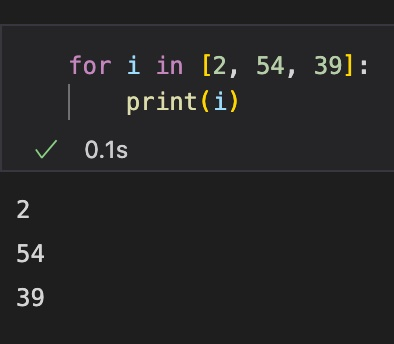
\includegraphics[width=3cm]{../images/illustrations/for.jpg}
      \end{figure}
   \end{minipage}
\end{frame}



\begin{frame}\frametitle{Essentials in the Python language}
   \begin{itemize}
      \item Functions
      \begin{itemize}
         \item A function can:
         \begin{itemize}
            \item take no, to many arguments
            \item arguments can be "Positional" or "Keyword" arguments
            \item return nothing (None) or anything (to many things)
            \item synonyms: arguments / parameters / inputs
         \end{itemize}
         \item One must:
         \begin{itemize}
            \item Define the function
            \item Call the function
         \end{itemize}
      \end{itemize}
   \end{itemize}
\end{frame}


\begin{frame}\frametitle{Functions}
   \begin{minipage}{0.38\linewidth}
      \begin{figure}[H]
         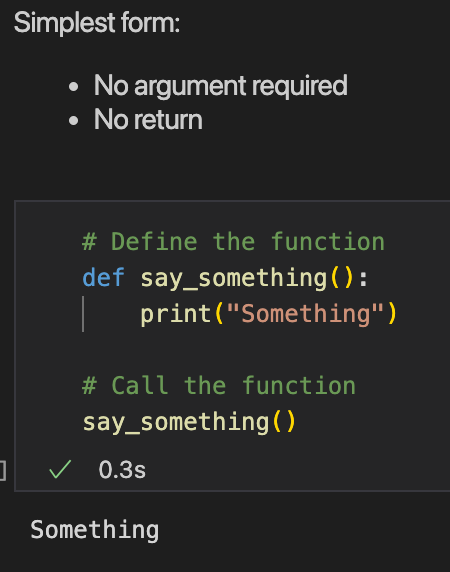
\includegraphics[width=3cm]{../images/illustrations/fct1.png}
      \end{figure}
      \begin{figure}[H]
         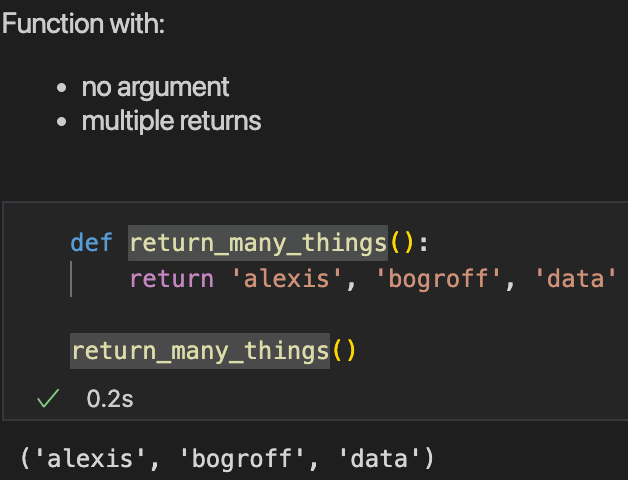
\includegraphics[width=4cm]{../images/illustrations/fct5.png}
      \end{figure}
   \end{minipage}
   \begin{minipage}{0.28\linewidth}
      \begin{figure}[H]
         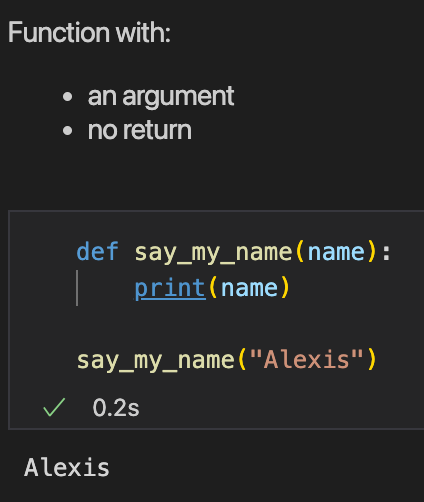
\includegraphics[width=2.7cm]{../images/illustrations/fct2.png}
      \end{figure}
      \begin{figure}[H]
         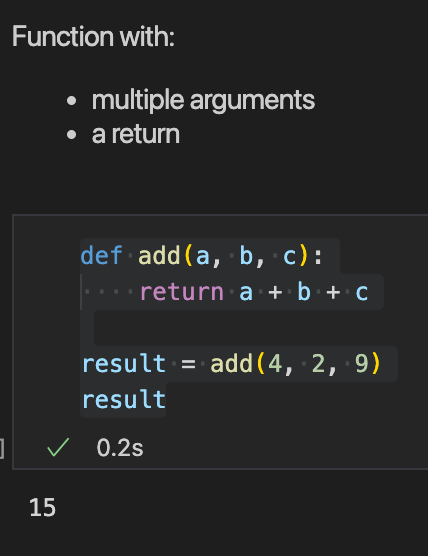
\includegraphics[width=2.8cm]{../images/illustrations/fct4.png}
      \end{figure}
   \end{minipage}
   \begin{minipage}{0.20\linewidth}
      \begin{figure}[H]
         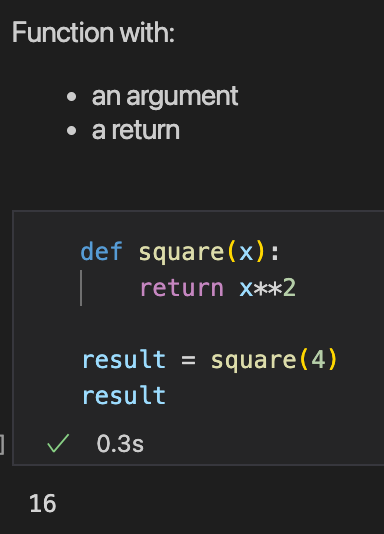
\includegraphics[width=2.5cm]{../images/illustrations/fct3.png}
      \end{figure}
      \begin{figure}[H]
         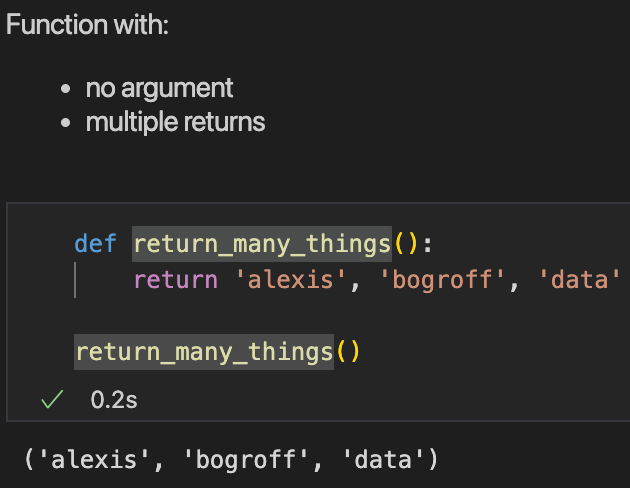
\includegraphics[width=4cm]{../images/illustrations/fct6.png}
      \end{figure}
   \end{minipage}
\end{frame}



\begin{frame}\frametitle{Functions}
   \begin{minipage}{0.48\linewidth}
      \begin{figure}[H]
         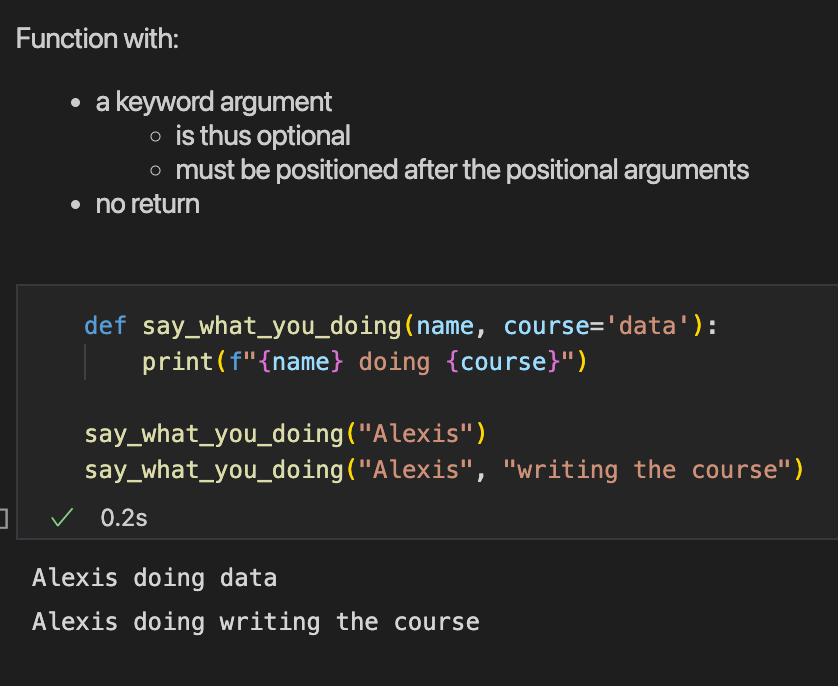
\includegraphics[width=5cm]{../images/illustrations/fct7.png}
      \end{figure}
   \end{minipage}
   \begin{minipage}{0.48\linewidth}
      \begin{figure}[H]
         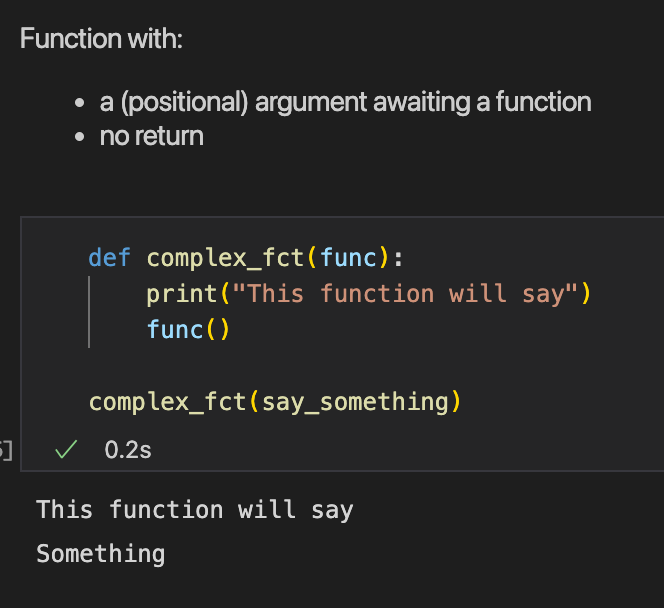
\includegraphics[width=4cm]{../images/illustrations/fct8.png}
      \end{figure}
   \end{minipage}
\end{frame}


\begin{frame}\frametitle{Objects - init}
   \begin{minipage}{0.3\linewidth}
      \begin{figure}[H]
         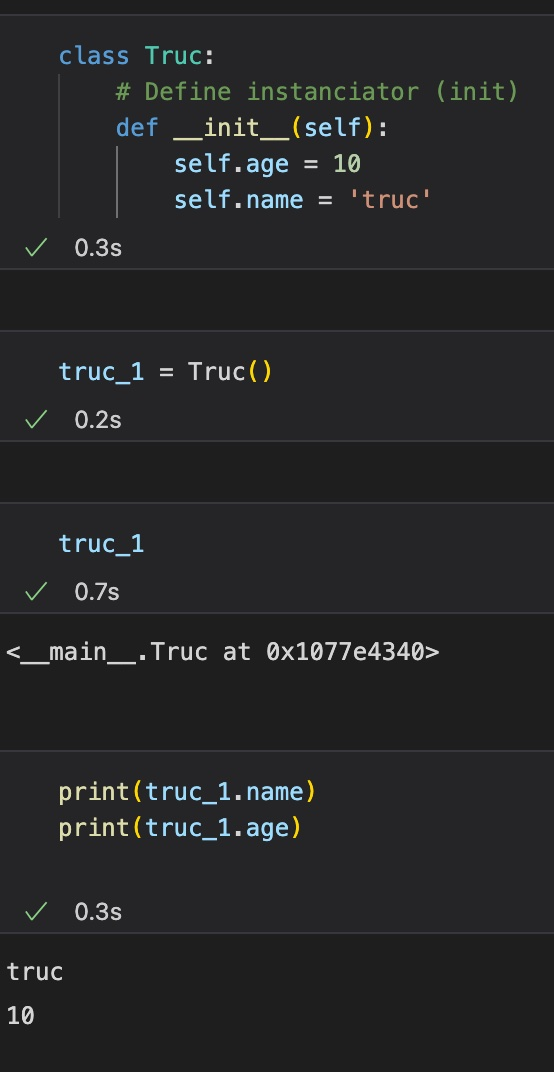
\includegraphics[width=3.2cm]{../images/illustrations/object_simple.jpg}
      \end{figure}
   \end{minipage}
   \begin{minipage}{0.68\linewidth}
      \begin{itemize}
         \item Define init
         \item Define properties / attributes (internal variables)
         \item Access through \textbf{self}
         \item Instanciate
         \item Object reference
         \item Access properties
      \end{itemize}
   \end{minipage}
\end{frame}

\begin{frame}\frametitle{Objects - method}
   \begin{minipage}{0.4\linewidth}
      \begin{figure}[H]
         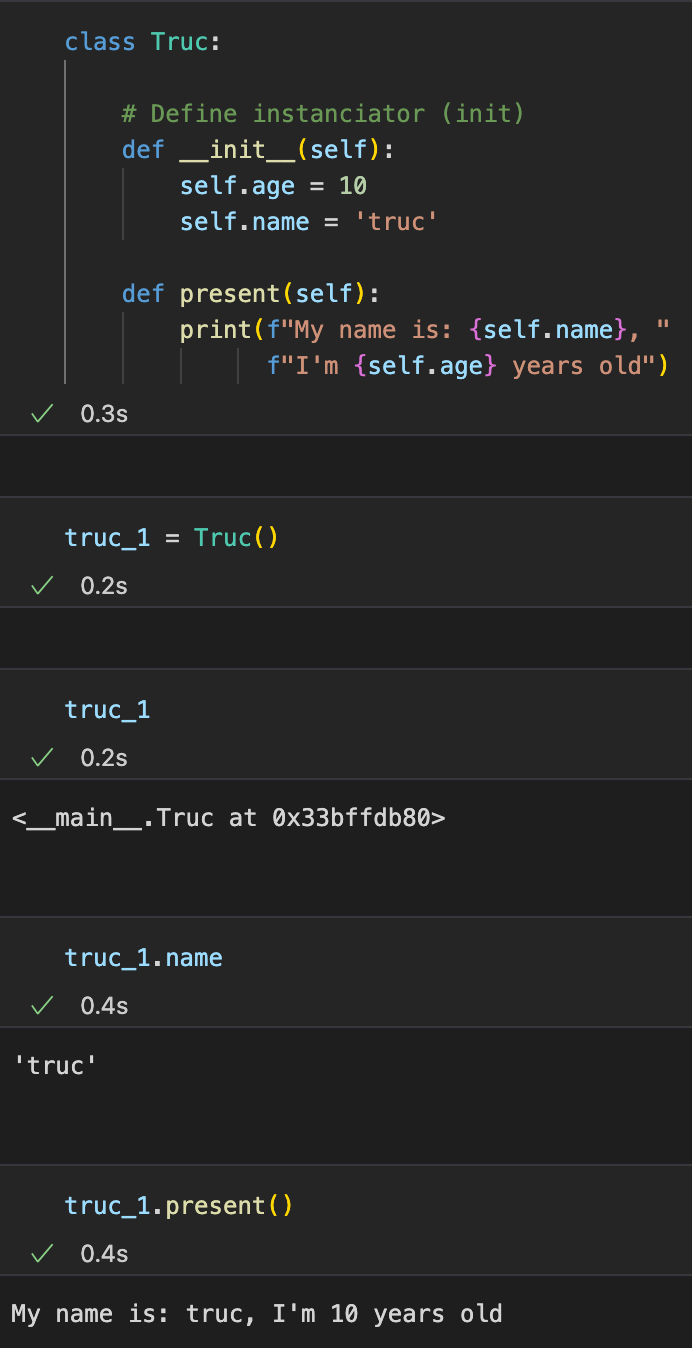
\includegraphics[width=4cm]{../images/illustrations/object_method.png}
      \end{figure}
   \end{minipage}
   \begin{minipage}{0.58\linewidth}
      \begin{itemize}
         \item Create method
         \item Pass \textbf{self} argument
         \item Access attributes via \textbf{self.attribute}
         \item Re-instanciate object \inlinegraphics{../images/illustrations/danger.png}
         \item New reference
         \item Access method via\\\textbf{self.method}
      \end{itemize}
   \end{minipage}
\end{frame}


\begin{frame}\frametitle{Objects - method with return}
   \begin{minipage}{0.4\linewidth}
      \begin{figure}[H]
         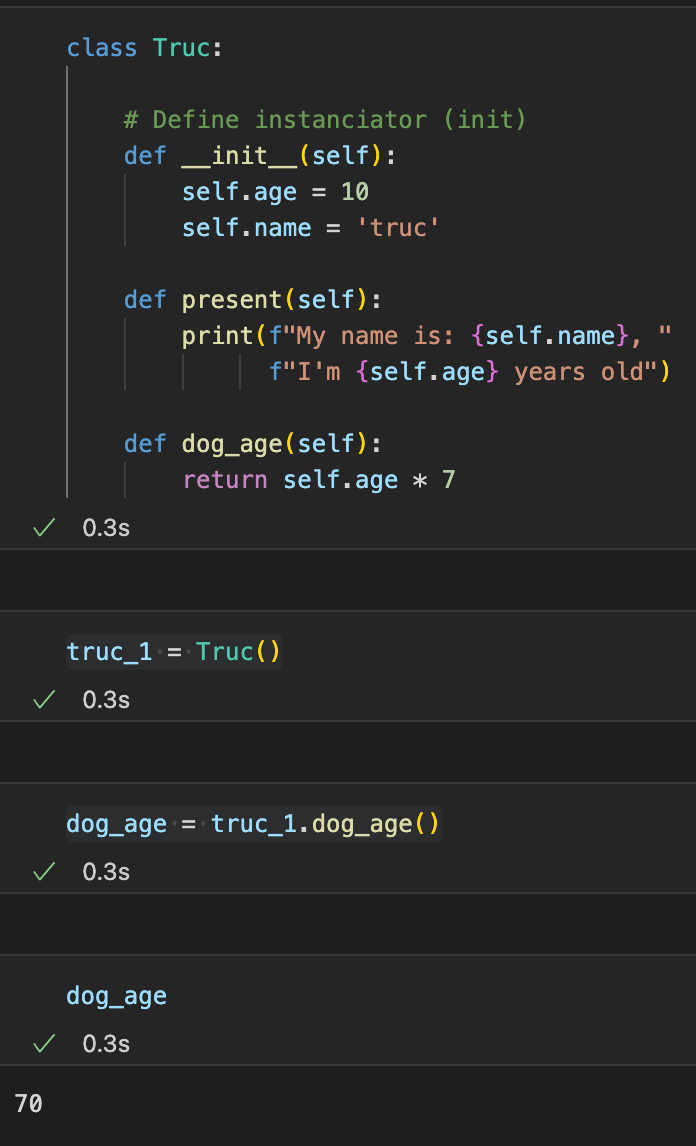
\includegraphics[width=4cm]{../images/illustrations/object_return.png}
      \end{figure}
   \end{minipage}
   \begin{minipage}{0.58\linewidth}
      \begin{itemize}
         \item Create method with return
         \item Set variable using return value
      \end{itemize}
   \end{minipage}
\end{frame}


\begin{frame}\frametitle{Objects - init with arguments}
   \begin{minipage}{0.48\linewidth}
      \begin{figure}[H]
         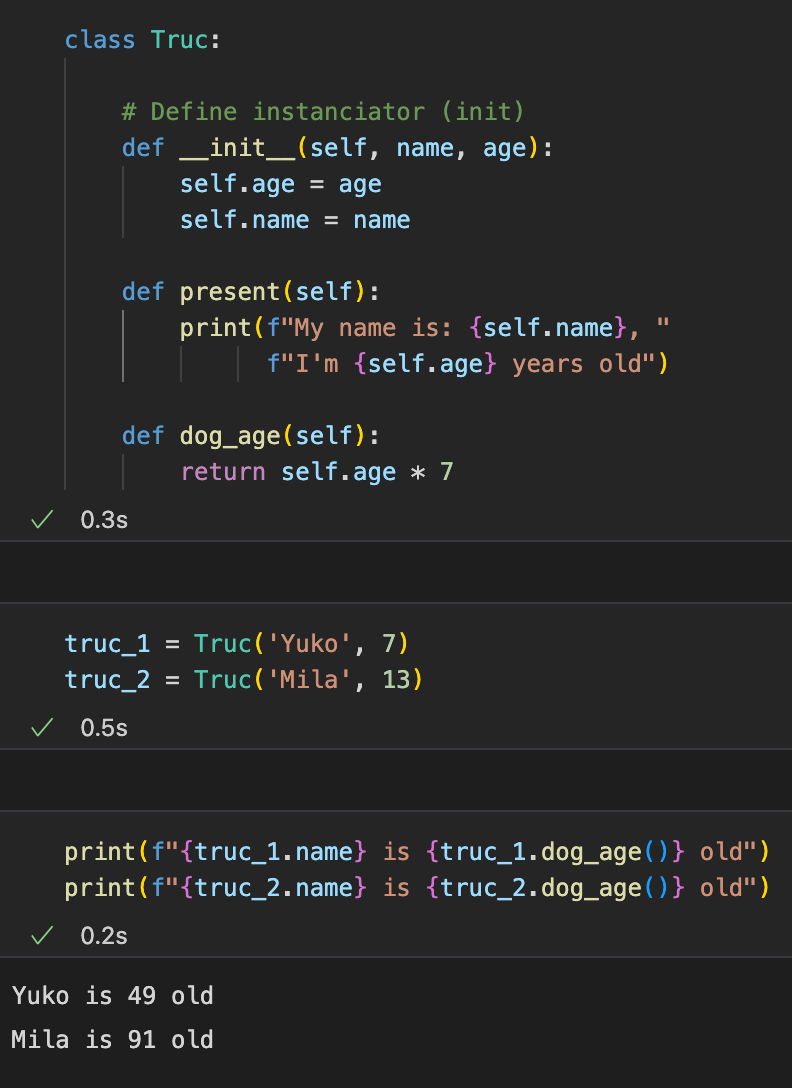
\includegraphics[width=4.8cm]{../images/illustrations/object_init_arguments.png}
      \end{figure}
   \end{minipage}
   \begin{minipage}{0.48\linewidth}
      \begin{itemize}
         \item Set specific init values
         \item Create different objects
      \end{itemize}
   \end{minipage}
\end{frame}


\begin{frame}\frametitle{Coding conventions}
   \begin{itemize}
      \item Names
      \begin{itemize}
         \item variables: snake\_style
         \item constants: CAPITAL\_SNAKE\_STYLE
         \item functions: snake\_style
         \item classes: First\_letter\_capital
      \end{itemize}
      \item Spaces
      \item Max number characters by row: \textbf{79}
      \item Creation of iterables (lists, dicts)
      \item Comments
      \item File, functions, classes description
   \end{itemize}
\end{frame}


\begin{frame}\frametitle{Coding conventions}
   \begin{itemize}
      \item Code order in a file:
      \begin{itemize}
         \item Description
         \item Imports
         \item Constants
         \item Functions and Classes alphabetically
         \item Body (functions calls, loops, variables)
      \end{itemize}
      \item Code organisation between files (script):
      \begin{itemize}
         \item Main file
         \item Functions and Classes file
         \item Settings file
      \end{itemize}
      \item Code organisation files (Jupyter Notebook):
      \begin{itemize}
         \item Load and prepare data file
         \item Analysis file
         \item Predictions file
      \end{itemize}
   \end{itemize}
\end{frame}

%------------------------------------------------------------------------------
\subsection{Programming in general}
%------------------------------------------------------------------------------

\subsubsection{Good Practices}

\begin{frame}\frametitle{Programming in general, good practices}
   \begin{figure}[H]
      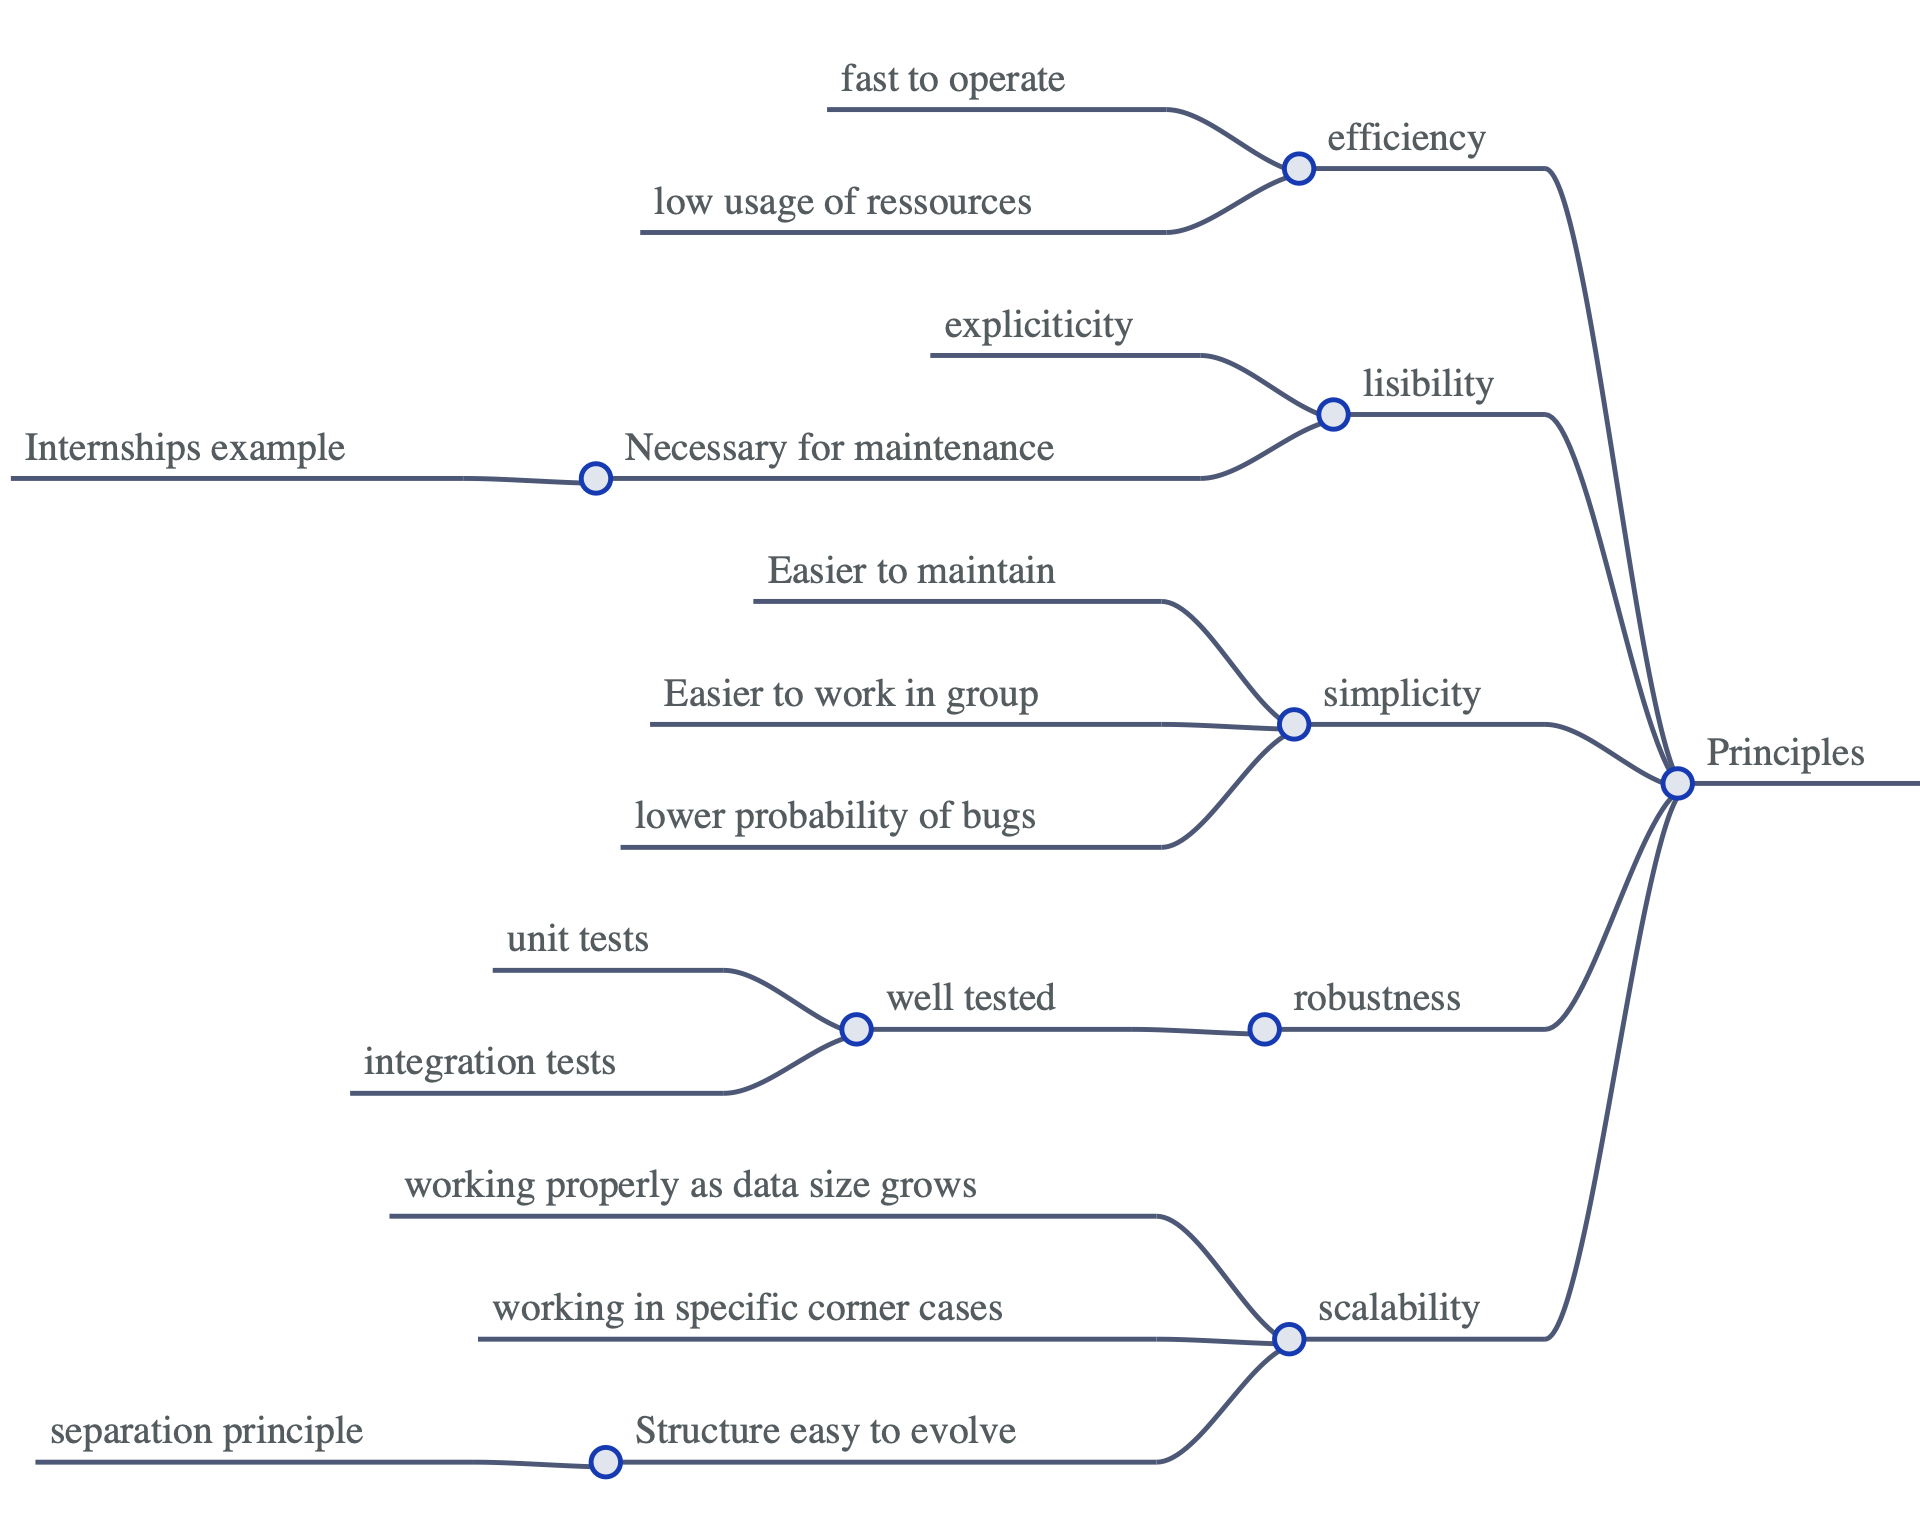
\includegraphics[width=9cm]{../images/illustrations/principles.png}
   \end{figure}
\end{frame}

\begin{frame}\frametitle{Programming in general, good practices}
   \begin{itemize}
      \item Vectorization
      \item Don't use loops when its possible to vectorize
      \item Same in Python, Matlab
      \item \textit{This code is explained in the next course}
   \end{itemize}

   \begin{figure}[H]
      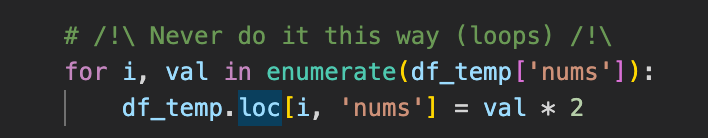
\includegraphics[width=5cm]{../images/illustrations/mult_loop.png}
   \end{figure}

   \begin{figure}[H]
      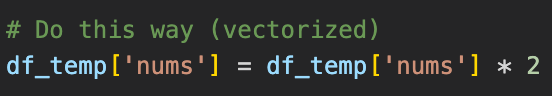
\includegraphics[width=4.2cm]{../images/illustrations/mult_vectorized.png}
   \end{figure}
\end{frame}


\subsubsection{Other languages}

\begin{frame}\frametitle{Programming in general, other languages}

   \begin{itemize}
      \item Difference between programming for:
      \begin{itemize}
         \item Analysis, statistics
         \item Software development
         \begin{itemize}
            \item Front-end
            \item Back-end
         \end{itemize}
      \end{itemize}
   \end{itemize}

\end{frame}

%------------------------------------------------------------------------------
\subsection{How to learn programming}
%------------------------------------------------------------------------------

\begin{frame}\frametitle{How to learn programming}
   \begin{itemize}
      \item Trial and error
      \item Could be enough at first:
      \begin{itemize}
         \item Python official documentation
         \item Exercises \href{https://www.codingame.com/home}{Coding game}
         \item Google, Stackoverflow, Blogs
      \end{itemize}
      
      \item Progress:
      \begin{itemize}
         \item Choose project (company, Kaggle, personal)
         \item Peers: open-source project, Data For Good
         \item MOOC: advanced course
      \end{itemize}
   \end{itemize}
\end{frame}

\end{document}
